\documentclass[12pt,chapterheads]{ucsd}
% documentclass options: default is 11pt, oneside, final.
% fonts: 10pt, 11pt, 12pt -- are valid for UCSD dissertations.
% sides: oneside, twoside -- note that two-sided theses are not accepted by OGS
% mode: draft, final -- draft mode switches to single spacing, removes hyperlinks,
%                       and places a black box at every overfull hbox (check these before submission).
% chapterheads -- include this if you want your chapters to read:
% Chapter 1
% Title of Chapter
%
% instead of
%
% 1 Title of Chapter

% Input and configure the required packages.
% UCSD Mathematics Dissertation Template
%
% Please read the comments in this file and make appropriate edits.
% NOTE: Always refer to the ``Preperation and Submission Manual for
% Doctoral Dissertations and Masters Theses for 20**'', where 20** is
% the year of your graduation, for officiation preparations guidelines.
%
% If you desire more control, please see the attached files:
%   * ucsd.cls -- Class file
%   * uct10.clo, uct11.clo, uct12.clo -- Configuration files for font sizes 10pt,11pt,12pt
%
% CHANGELOG:
%   * Original file adapted from brockman.tex by JRB and RMR
%     to work with ucsd.cls

% Include all packages you need here.  Some standard options are suggested below.

% GEOMETRY - This will force the use of Letter paper.
% Many TeX installations default to A4 paper.  The formatting
% of the thesis class file requires Letter, else the margins
% will be wrong when you go to print it (and OGS will complain).
% If your TeX implementation is not setup for Letter paper, and
% you cannot change it, uncommenting the following line may fix
% problem.
% \usepackage[paper=letterpaper]{geometry}


%% AMS PACKAGES - Chances are you will want some or all of these if writing a math dissertation.
% \usepackage{amsmath, amscd, amssymb, amsthm}

%% GRAPHICX - This is the standard package for including graphics for latex/pdflatex.
% \usepackage{graphicx}

%% LATIN MODERN FONTS (replacements for Computer Modern)
% \usepackage{lmodern}
% \usepackage[T1]{fontenc}

%% INDEX
% Uncomment the following two lines to create an index:
% \usepackage{makeidx}
% \makeindex
% You will need to uncomment the \printindex line near the
% bibliography to display the index.  Use the command
% \index{keyword} within the text to create an entry in the index
% for keyword.

%% HYPERLINKS
% To create a PDF with hyperlinks, you need to include the hyperref package.
% THIS HAS TO BE THE LAST PACKAGE INCLUDED!
% Note that the options plainpages=false and pdfpagelabels exist
% to fix indexing associated with having both (ii) and (2) as pages.
% Also, all links must be black according to OGS.
% See: http://www.tex.ac.uk/cgi-bin/texfaq2html?label=hyperdupdest
% Note: This may not work correctly with all DVI viewers (i.e. Yap breaks).
% NOTE: hyperref will NOT work in draft mode, as noted above.
% \usepackage[colorlinks=true, pdfstartview=FitV, linkcolor=black, citecolor=black, urlcolor=black,plainpages=false,pdfpagelabels]{hyperref}
% \hypersetup{ pdfauthor = {Your Name Here}, pdftitle = {The Title of The Dissertation}, pdfkeywords = {Keywords for Searching}, pdfcreator = {pdfLaTeX with hyperref package}, pdfproducer = {pdfLaTeX}}

\usepackage{amsmath,amsfonts,amsthm,amssymb}
\usepackage{setspace}
\usepackage{fancyhdr}
\usepackage{lastpage}
\usepackage{extramarks}
\usepackage{chngpage}
\usepackage{soul}
\usepackage[usenames,dvipsnames]{color}
\usepackage{graphicx,float,wrapfig}
\usepackage{subfig}
\usepackage{ifthen}
\usepackage{listings}
\usepackage{courier}
\usepackage{microtype}
\usepackage{appendix}
\usepackage{hyperref}
\usepackage[all]{hypcap}
\usepackage{url}
\usepackage{algorithmic}
\usepackage{booktabs}
\usepackage{cancel}

% Needed for changing the font size in \documentclass{} while
% using the fancyhdr package. Else the warning:
% \headheight is too small (12.0pt):Make it at least 14.49998pt.
\setlength{\headheight}{15pt}

% For faster processing, load Matlab syntax for listings
\definecolor{MyDarkGreen}{rgb}{0.0,0.4,0.0}
\lstloadlanguages{Matlab}%
\lstset{language=Matlab,
       frame=single,
       basicstyle=\scriptsize\ttfamily,
       keywordstyle=[1]\color{Blue}\bf,
       keywordstyle=[2]\color{Purple},
       keywordstyle=[3]\color{Blue}\underbar,
       identifierstyle=,
       commentstyle=\usefont{T1}{pcr}{m}{sl}\color{MyDarkGreen}\small,
       stringstyle=\color{Purple},
       showstringspaces=false,
       tabsize=5,
       % Put standard MATLAB functions not included in the default
       % language here
       morekeywords={xlim,ylim,var,alpha,factorial,poissrnd,normpdf,normcdf},
       % Put MATLAB function parameters here
       morekeywords=[2]{on, off, interp},
       % Put user defined functions here
       morekeywords=[3]{FindESS},
       morecomment=[l][\color{Blue}]{...},
       numbers=left,
       firstnumber=1,
       numberstyle=\tiny\color{Blue},
       stepnumber=0
       }

% Adds a hyperlink to an email address.
\newcommand{\mailto}[2]{\href{mailto:#1}{#2}}

% Homework Specific Information
\newcommand{\thesisTitle}{Lyapunov Variable Comparison}
\newcommand{\thesisSubTitle}{}
\newcommand{\thesisAuthorName}{Thomas Denewiler}
\newcommand{\thesisAuthorEmail}{tdenewiler@gmail.com}

% These commands set the document properties for the PDF output. Needs the hyperref package.
\hypersetup
{
    colorlinks,
    linkcolor={black},
    citecolor={black},
    filecolor={black},
    urlcolor={black},
    pdfauthor={\thesisAuthorName <\mailto{\thesisAuthorEmail}{\thesisAuthorEmail}>},
    pdfsubject={\thesisTitle},
    pdftitle={\thesisTitle},
    pdfkeywords={UC San Diego, Small Unmanned Ground Vehicles, Robotics},
    pdfstartpage={1},
}

% Includes a MATLAB script.
% The first parameter is the label, which also is the name of the script.
% The second parameter is the optional caption.
\newcommand{\matlabscript}[2]
  {\begin{itemize}\item[]\lstinputlisting[caption=#2,label=#1]{#1}\end{itemize}}

% User defined macros.
\def\argmin{\mathop{\arg\,\min}\limits}
\def\argmax{\mathop{\arg\,\max}\limits}
\def\argsol{\mathop{\arg\,\text{sol}}\limits}
\def\atanh{\mathop{\text{atanh}}}


% Uncomment this to add line numbers for debugging only.
\usepackage{lineno}
\def\linenumberfont{\normalfont\small\sffamily}
\linenumbers

% Uncomment this line to compile a subset of the chapters.
\includeonly{chapters/chEstimation}

% Document starts here.
\begin{document}

% Document specific information.
%% REQUIRED FIELDS -- Replace with the values appropriate to you
\title{Robot Traffic School}
% No symbols, formulas, superscripts, or Greek letters are allowed
% in your title.

\author{Thomas Denewiler}
\degreeyear{2010}
\degree{Master's of Science}
% Master's Degree theses will NOT be formatted properly with this
% file.

\field{Mechanical and Aerospace Engineering}
\chair{Professor Thomas Bewley}
% Uncomment the next line iff you have a Co-Chair
% \cochair{Professor Cochair Semimaster}
% \othermembers{%  These must be alpha by last name.
% Professor Humor Less\\
% Professor Ironic Name\\
% Professor Cirius Thinker\\
% }
\numberofmembers{1} % |chair| + |cochair| + |othermembers|

% The title, copyright, and signature pages.
\begin{frontmatter}
% \makefrontmatter
% No symbols, formulas, superscripts, or Greek letters are allowed
% in your title.
\title{Robot Traffic School: Improving Autonomous Navigation in EOD Robots}
\author{Thomas Denewiler}
\degreeyear{2011}
\degree{Master of Science}
\field{Engineering Sciences (Mechanical Engineering)}
\chair{Professor Thomas R. Bewley}

% Uncomment the next line iff you have a Co-Chair
% \cochair{Professor Cochair Semimaster} 
%
% Or, uncomment the next line iff you have two equal Co-Chairs.
%\cochairs{Professor Chair Masterish}{Professor Chair Masterish}

%  The rest of the committee members  must be alphabetized by last name.
\othermembers{
Professor Raymond de Callafon \\ 
Professor Ryan Kastner \\
}
\numberofmembers{3} % |chair| + |cochair| + |othermembers|

%% START THE FRONTMATTER
\makeatletter
\let\@currsize\normalsize
\begin{frontmatter}
\makefrontmatter

%% DEDICATION
% You have three choices here:
%   1. Use the ``dedication'' environment.   Put in the text you want,
%   and you'll get a perfectly respectable dedication page.
%
%   2. Use the ``mydedication'' environment.  If you don't like the
%   formatting of option 1, use this environment and format things
%   however you wish.
%
%   3. If you don't want a dedication, it's not required.
\begin{dedication} % The style file will format this for you.
To Grandma Denny, \\
it's a small step from board games to Kalman filters, \\
To my parents, \\
for their time and encouragement in everything.
\end{dedication}

% \begin{mydedication} % You are responsible for formatting here.
%   \vspace{1in}
%   \begin{flushleft}
% 	To me.
%   \end{flushleft}
%
%   \vspace{2in}
%   \begin{center}
% 	And you.
%   \end{center}
%
%   \vspace{2in}
%   \begin{flushright}
% 	Which equals us.
%   \end{flushright}
% \end{mydedication}


%% EPIGRAPH
%  The same choices that applied to the dedication apply here.

% \begin{epigraph} % The style file will position the text for you.
%   \emph{A careful quotation\\
%   conveys brilliance.}\\
%   ---Smarty Pants
% \end{epigraph}

% \begin{myepigraph} % You position the text yourself.
%   \vfil
%   \begin{center}
%     {\bf Think! It ain't illegal yet.}
%
% 	\emph{---George Clinton}
%   \end{center}
% \end{myepigraph}

\tableofcontents
\listoffigures  % Uncomment if you have any figures
\listoftables   % Uncomment if you have any tables


%% ACKNOWLEDGEMENTS
%  While technically optional, you probably have someone to thank.
%  Also, a paragraph acknowledging all coauthors and publishers (if
%  you have any) is required in the acknowledgements page and as the
%  last paragraph of text at the end of each respective chapter. See
%  the OGS Formatting Manual for more information.

\begin{acknowledgements}
The enthusiasm and energy of Professor Thomas Bewley has been an inspiration and his support and advice have been invaluable.

I am grateful to Gideon Prior, Nima Ghods, Amin Rahimi and Steve Stancliff for our many long conversations while learning how to build better robots.

I would also like to thank Mike Bruch, Bart Everett and the ACS team (Gaurav Ahuja, Donnie Fellars, Greg Kogut and Brandon Sights) as well as Jason Lum, Kelly Grant and the EOD technicians at SPAWAR for their support with both hardware and software.

And without the love and encouragement from Silvie Georgens I would not have made it this far.
\end{acknowledgements}


%% VITA
%  A brief vita is required in a doctoral thesis. See the OGS
%  Formatting Manual for more information.
% \begin{vitapage}
% \begin{vita}
%   \item[2002] B.~S. in Mathematics \emph{cum laude}, University of Southern North Dakota, Hoople
%   \item[2002-2007] Graduate Teaching Assistant, University of California, San Diego
%   \item[2007] Ph.~D. in Mathematics, University of California, San Diego
% \end{vita}
% \begin{publications}
%   \item Your Name, ``A Simple Proof Of The Riemann Hypothesis'', \emph{Annals of Math}, 314, 2007.
%   \item Your Name, Euclid, ``There Are Lots Of Prime Numbers'', \emph{Journal of Primes}, 1, 300
% 	B.C.
% \end{publications}
% \end{vitapage}

%% Abstract
% Doctoral dissertation abstracts should not exceed 350 words. MS thesis
% abstracts can be up to 250 words. The abstract may, however, continue to a
% second page if necessary.
% Keep a blank line after \begin{abstract} and the first line of the abstract so that indentation occurs.
\begin{abstract}

Advancements in the autonomous navigation of robots increases the range of behaviors that can be implemented, consequently increasing the utility of the robots to end users. To achieve these advancements, the state estimation and controls algorithms for Explosives Ordinance Disposal (EOD) robots have been studied and improved. In this work, I integrated a high precision, differential GPS system to measure ground truth positions, which were then used to find more accurate system and measurement noise covariance values. The more accurate noise models improved the state estimate of an extended Kalman filter. Independently, a model-based control law was implemented for a vehicle with nonholonomic unicycle constraints kinematics using a Lyapunov method. The Lyapunov controller was implemented on several different EOD robots and is compared to the previously existing PID controller with respect to navigation near simulated obstacles and in open space. Practical considerations for tuning the Lyapunov controller design variables are explored, and recommendations are given for several operating scenarios. The improved algorithms were implemented using multiple different robots. The algorithms are currently running on EOD robots used in the field. This work will accelerate development of advanced maneuvers, such as retroverse over long distances as well as obstacle avoidance.
\end{abstract}

\end{frontmatter}
\makeatother

\end{frontmatter}

% Meat and potatoes.
\chapter{Introduction}
Robots have been developed to assist humans in tasks that are generally considered dirty, dangerous or boring. Recently robots have found a useful niche as a tool to help Expolosives Ordinance Disposal (EOD) teams to assess and eliminate threats due to improvised explosive devices (IEDs), commonly referred to as roadside bombs, by allowing humans to maintain a safe stand-off distance while investigating a scene. Clearly this falls under the dangerous category. The current method that EOD teams use involves teleoperation of the robot to get from the base to the object of interest. In the process of teleoperating the robot the operator is exposed and vulnerable to other external threats in the area. As technologies mature to provide humans with better tools shortcomings are discovered, such as the vulnerability due to teleoperation, and that opens up avenues for improvement in the development of these tools. For robots one approach to reducing the amount of work humans are required to perform is to give the robots more intelligence via autonomous behaviors using additional sensors, more specialized actuators and software to automate the largest amount of routine tasks as possible.

When adding autonomy to robots nearly all of the tasks can be summarized by the following questions:
\begin{itemize}
\item Where am I?
\item What's around me?
\item Where do I want to go?
\item How do I get there?
\end{itemize}

The initial attempt at adding autonomy to the EOD robots resulted in somewhat erratic driving behavior, especially near obstacles, as the robot trajectory would be very jerky *** needs a better description *** when it changed speed and attempted to make small corrections to its original path to move around the obstacle. In this paper I will look at smoothing out the trajectories taken by the robot by looking for improvements in the state estimation (Where am I?) and controls (How do I get there?) algorithms. For this work I am ignoring actual obstacle detection (What's around me?) and will be using a simple planning algorithm (Where do I want to go?) to simulate obstacles in the robot path which will force the robot to change direction and speed multiple times.

*** Talk more about how this problem is not isolated to any one issue and that state estimation, control and sensor measurements all need to be considered. I need to show later how each piece contributes to making the robot drive better. ***
\chapter{Background}
\label{ch:background}
*** Put in a description of the PackBot, Talon and Urbot along with a description of the algorithms originally used and the results obtained using those algorithms. Talk about JAUS and MOCU a little bit. Discuss more about how the robots are used by EOD. Include that for robots to drive around on their own all they require is an estimate of where they are, a path to follow, a controller to determine the actuator outputs and motor controllers to perform the controller outputs. ***

*** It might be best to have more of a description of the actual problem here along with a description of the testing area. ***

\section{Small Unmanned Ground Vehicles}
\label{sec:smallugvs}
The PackBot is manufactured by iRobot. *** Add more. ***

The Talon is manufactured by Foster Miller. *** Add more. ***

The Urbot is an experimental prototype of a small UGV developed by SSC-SD and is shown in Figure \ref{fig:urbot}. *** Add more. ***

*** Say that each of the robots has a standard sensor suite and list what those sensors are. ***

\begin{figure}[ht!]
	\centering
	\includegraphics[width=.5\textwidth]{images/urbot}
	\caption{Urbot.}
	\label{fig:urbot}
\end{figure}

\section{MOCU \& JAUS}
\label{sec:mocujaus}
The Multi-Robot Operator Control Unit (MOCU) is a highly configurable front-end for simultaneous command and control of multiple systems and was created at SSC-SD \cite{PowellMOCU08}. MOCU has the ability to use a variety of communications protocols for interfacing to different systems and uses the Joint Architecture for Unmanned Systems (JAUS) to send and receive data to all of the UGVs used in this research \cite{RoweJAUS08}.

\section{The Duals: Estimation \& Controls}
\label{sec:duals}
It is very difficult to simply work on either state estimation or controls individually as there is a large amount of coupling between the two areas. Although the main goal is to make the robots drive more smoothly and the actuator and motor outputs are ultimately generated by the control system it is still the case that the role of state estimation is equally important. If there exist large meaurement errors, drift or bias in the sensor readings then the robot will not have a very good idea of where it is locted and there will not be a controller that can stabilize the system. *** Talk about observability and controllability. Mention theory that shows link between estimation and control. ***

An example would be when the only sensor available for measurements is an IMU which suffers from drift and bias, where both effects are exagerrated by temperature. There have been situations in which an IMU was in a robot with the motors turned off so that the robot is not moving. However, due to excessive heat in the electronics bos the IMU measurements report that the heading of the robot keeps moving in circles at a rate of $\frac{\pi}{5} rad/s$. With a controller that was known to keep the robot stable when the IMU was working properly started forcing the robot to turn in circles when the motors were turned on even thought the command was to stay in one place. This shows the importance of state estimation on overall robot performance -- it is not enough to only have a good controller.
\chapter{State Estimation}
\label{ch:estimation}
*** Talk about quantifying the performance of the ACS Kalman filter \cite{Sights06}. Discuss training of the covariance matrices. Show the position estimation using the original covariance matrices and the ones found from training. If I get to identifying bias and/or drift in the IMU put that here as well. ***

The Space and Naval Warfare Systems Center, San Diego (SSC-SD) robotics group has developed the Autonomous Capabilities Suite (ACS) which incorporates many different technologies into a single software package that can be run on a wide variety of different robots and is able to easily accomodate different payload and sensor suites \cite{Sights06}. One of the ACS libraries is the adaptive extended Kalman filter which is used on the EOD robots for state estimation and is the main method used for answering the question ``Where am I?''. The idea behind the Kalman filter is relatively straightforward. The robot has some basic idea of where it is in the world but there is some uncertainty involved in that estimate due to different measurement accuracies from multiple sensors that measure the same state, noise in the individual sensor measurements and an imperfect model of how the robot moves through the world. Some of the uncertainty of the model can be explained by the fact that not all of the necessary measurements are being carried out and the states can be unobservable. *** Say more here about noise/uncertainty. ***

An example is a robot driving in a straight line where the left track may be moving on a flat surface while the right track is moving on an uneven surface as in Figure \ref{fig:topography}. The wheel encoders that measure how far each track is moving will report that the right track is traveling a greater distance than the left track which could mean that the robot is turning counter-clockwise or that the robot tracks are moving over different surface types. At the same time the robot will be getting measurements about its heading from both the IMU and GPS sensors that will have some noise as well. In this example both the IMU and GPS sensors would likely say that the robot is traveling in a straight line on average (as long as the controller is performing adequately). The job of the Kalman filter is to determine how much each sensor should be trusted when trying to determine where the robot really is in the world and how fast it is moving. This is accomplished by looking at each of the noise parameters for both the system model and the measurements as being zero mean, white noise, uncorrelated, Gaussian variables ... *** Clean up this language. Consider putting it in a different section like \S\ref{sec:duals}. ***

\begin{figure}[ht!]
	\centering
	\includegraphics[width=.5\textwidth]{images/topography}
	\caption{Different topographies for the left track and the right track when the ground is smooth on the left side and bumpy on the right side. The top line is for the left track and the bottom line is for the right track.}
	\label{fig:topography}
\end{figure}

\section{State Space Models}
\label{sec:statespacemodels}
Kalman filters and control systems (see Chapter \ref{ch:controls}) use the idea of a multi-dimensional state space to encapsulate all of the relevant information that is known about a system. In the case of robots the dynamics are typically captured by position, orientation, linear and angular velocities, acceleration and sometimes jerk. The general equations to describe the state space of a system are

\begin{align}
\label{eq:statespace}
\begin{split}
\dot{x} &= f(x,u,t) \\
\dot{y} &= h(x,t)
\end{split}
\end{align}

The state variables are given in vector form by $x$ and the sensor measurements are contained in the vector $y$. The state space equations are a means of representing how the state and measurements of a system change through time based on the initial state of the system and the inputs, $u$, to the system which allows the trajectory (or motion through time) and the effect of the trajectory on the measurements to be calculated using compact notation. The inputs are assumed to include any external forces applied to the system as well as actuation provided by the system itself.

\section{The Kalman Filter}
\label{sec:kalmanfilter}
The ACS Kalman filter is typical of all Kalman filters in that it consists of a prediction update step and a measurement update step where the prediction update is run as fast as possible and the measurement update is run whenever new sensor data becomes available as in Figure \ref{fig:kf}. The prediction update step uses a model of the system dynamics and a measurement of elapsed time to determine where the system is in the world and will inevitably have errors due to effects that are not captured by the model, especially when the system dynamics are linearized. The measurement update step is basically a feedback step to help correct for errors in the system model using sensors to provide current data \cite{Kelly_1994_338}.

\begin{figure}[ht!]
	\centering
	\includegraphics[width=.4\textwidth]{images/kf}
	\caption{The Kalman filter algorithm.}
	\label{fig:kf}
\end{figure}

The Kalman filters that run on the small UGVs used in these experiments run on digital computers and are necessarily discretized forms because of the nature of computers. From \cite{Kelly_1994_338}, \cite{Simon06OptimalEstimation} the discretized versions of (\ref{eq:statespace}) mean that the state space equations are

\begin{align}
\label{eq:kfstatemodel}
\begin{split}
x_{k+1} &= \Phi_kx_k + \Gamma_kw_k \\
y_k &= H_kx_k + v_k
\end{split}
\end{align}
where $\Phi_k$ is the state transition matrix relating the state at time $k+1$ to time $k$ in the absence of inputs including noise, $\Gamma_k$ is the noise distribution matrix which translates the input vector $w_k$ into the coordinates of the state, $H_k$ is the measurement matrix which relates the measurements to the state vector and $v_k$ is the sensor measurement noise.

The prediction update step marches the system dynamics forward in time using the equations

\begin{align}
\label{eq:kfpredictionupdate}
\begin{split}
\hat{x}_{k+1}^- &= \Phi_k\hat{x}_k^+ \\
P_{k+1}^- &= \Phi_kP_k^+\Phi_k^T + \Gamma_kQ_k\Gamma_k^T
\end{split}
\end{align}
and the measurement update step provides feedback from sensor data using the equations

\begin{align}
\label{eq:kfmeasurementupdate}
\begin{split}
K_k &= P_k^-H_k^T\left[H_kP_k^-H_k^T + R_k\right]^{-1} \\
\hat{x}_k^+ &= \hat{x}_k^- + K_k\left[y_k - H_k\hat{x}_k^-\right] \\
P_k^+ &= \left[I - K_kH_k\right]P_k^-
\end{split}
\end{align}

The prediction update step relies on knowing $\Phi_k$, $\Gamma_k$ and the disturbance covariance matrix, $Q_k$, while the measurement update step needs to know $H_k$ and the measurement covariance matrix, $R_k$. Using (\ref{eq:kfpredictionupdate}) and (\ref{eq:kfmeasurementupdate}) an estimate of the state of the robot can be obtained at any time for use by the controls algorithms.

\subsection{Extended Kalman Filter}
\label{sec:extendedkf}
The basic Kalman filter makes the assumption that both the system model contained in $\Phi_k$ and the measurement model in $H_k$ are linear. The extended Kalman filter (EKF) allows for nonlinear models to be used for $\Phi_k$, $H_k$ or both by linearizing the models around the state estimate. *** Talk about how partial derivatives are used to linearize the models. ***

The state vector used in the ACS EKF follows that found in \cite{Kelly_1994_338}, \cite{Kelly_1994_333} which avoids issues of non-observability by using the principal motion assumption where

\begin{align*}
x_k = \left[\begin{array}{c c c c c c c c} x & y & z & v & \theta & \phi & \psi & \omega \end{array}\right]^T
\end{align*}
In this vector $x$, $y$ and $z$ are positions, $v$ is velocity, $\theta$, $\phi$ and $\psi$ are Euler angles for pitch, roll and yaw, and $\omega$ is angular velocity. The state transition matrix is

\begin{align*}
\Phi_k = \left[\begin{array}{c c c c c c c c}
1 & 0 & 0 & \cos(\psi)*\cos(\theta)*\Delta T & 0 & 0 & 0 & 0 \\
0 & 1 & 0 & \sin(\psi)*\cos(\theta)*\Delta T & 0 & 0 & 0 & 0\\
0 & 0 & 1 & -\sin(\theta)*\Delta T & 0 & 0 & 0 & 0\\
0 & 0 & 0 & 1 & 0 & 0 & 0 & 0 \\
0 & 0 & 0 & 0 & 1 & 0 & 0 & -\sin(\phi)*\Delta T \\
0 & 0 & 0 & 0 & 0 & 1 & 0 & \tan(\theta)*\cos(\phi)*\Delta T \\
0 & 0 & 0 & 0 & 0 & 0 & 1 & \cos(\phi)*\Delta T/\cos(\theta)\\
0 & 0 & 0 & 0 & 0 & 0 & 0 & 1
\end{array}\right]
\end{align*}
The process noise matrix is

\begin{align*}
\Gamma_k = \left[\begin{array}{c c c c c c c c}
\Gamma_{1,1} & \Gamma_{1,2} & \Gamma_{1,3} & 0 & 0 & 0 & 0 & 0 \\
\Gamma_{2,1} & \Gamma_{2,2} & \Gamma_{2,3} & 0 & 0 & 0 & 0 & 0 \\
\Gamma_{3,1} & \Gamma_{3,2} & \Gamma_{3,3} & 0 & 0 & 0 & 0 & 0 \\
0 & 0 & 0 & 1 & 0 & 0 & 0 & 0 \\
0 & 0 & 0 & 0 & \cos(\phi) & 0 & \sin(\phi) & 0 \\
0 & 0 & 0 & 0 & -\tan(\theta)*\sin(\phi) & 1 & \tan(\theta)*\cos(\phi) & 0 \\
0 & 0 & 0 & 0 & -\sin(\phi) / \cos(\theta) & 0 & \cos(\phi)/\cos(\theta) & 0 \\
0 & 0 & 0 & 0 & 0 & 0 & 0 & 1
\end{array}\right]
\end{align*}

where the upper left $3\times 3$ block matrix elements are

\begin{align*}
\Gamma_{1,1} &= \sin(\psi)*\cos(\phi)-\cos(\psi)\sin(\theta)*\sin(\phi) \\
\Gamma_{1,2} &= \cos(\psi)*\cos(\theta) \\
\Gamma_{1,3} &= \sin(\psi)*\sin(\phi)+\cos(\psi)*\sin(\theta)*\cos(\phi) \\
\Gamma_{2,1} &= -\cos(\theta)*\cos(\phi)-\sin(\theta)\sin(\theta)*\sin(\phi) \\
\Gamma_{2,2} &= \sin(\psi)*\cos(\theta) \\
\Gamma_{2,3} &= -\cos(\psi)*\sin(\phi)-\sin(\psi)*\sin(\theta)*\cos(\phi) \\
\Gamma_{3,1} &= -\cos(\theta)*\sin(\phi) \\
\Gamma_{3,2} &= -\sin(\theta) \\
\Gamma_{3,3} &= \cos(\theta)*\cos(\phi)
\end{align*}

\subsection{Adaptive Extended Kalman Filter}
\label{sec:adaptiveekf}
*** Discuss why $Q$ and $R$ are important and what function they serve in the Kalman filter. Why is it valid to update $Q$ and $R$ this way? ***

Attempting to determine the proper values for the covariance matrices $Q$ in (\ref{eq:kfpredictionupdate}) and $R$ in (\ref{eq:kfmeasurementupdate}) can be a laborious process and is often considered more of an art than a science with engineer experience being a critical factor.

The ACS Kalman filter has been implemented with an adaptive scheme to update the covariance matrices in real time as the robot moves around and sensor measurements are taken into account \cite{Sights06}, \cite{Mehra72}, \cite{Busse03adaptiveEKF}. Estimates of $Q$ and $R$ are updated at alternating time steps in the EKF. Recall from (\ref{eq:kfpredictionupdate}) and (\ref{eq:kfmeasurementupdate}) that $\hat{x}_k^+$ and $P_k^+$ are known after the measurement update step and $\hat{x}_k^-$ and $P_k^-$ are known after the system update step in the Kalman filter.

The first step is to calculate $Q^\star$ using

\begin{align}
\label{eq:qstar}
Q^\star = \left(\hat{x}_k^+-\hat{x}_k^-\right)\left(\hat{x}_k^+-\hat{x}_k^-\right)^T + P_k^- - P_k^+ - \hat{Q}_k^-
\end{align}
Then the estimate of $Q$ can be updated using

\begin{align}
\label{eq:qadapt}
\hat{Q}_k^+ = \hat{Q}_k^- + \frac{1}{L_Q}\left(Q^\star-\hat{Q}_k^-\right)
\end{align}

Next $R^\star$ is calculated using

\begin{align}
\label{eq:rstar}
R^\star = \left(y_k-\hat{y}_k^+\right)\left(y_k-\hat{y}_k^+\right)^T - H_kP_k^+H_k^T
\end{align}
where $y_k$ are actual measurement data and $\hat{y}_k^+ = h_k\hat{x}_k^+$ is calculated after the measurement update step. Then the estimate of $R$ can be updated using

\begin{align}
\label{eq:radapt}
\hat{R}_k^+ = \hat{R}_k^- + \frac{1}{L_R}\left(R^\star-\hat{R}_k^-\right)
\end{align}

*** Discuss the implications of the adaptive EKF. ***

\section{Establishing Ground Truth}
\label{sec:groundtruth}
Quantitatively evaluating the performance of Kalman filters can be done accomplished in several ways, the best of which is to analyze the output of the Kalman filter against ground truth. Although it is nearly impossible to establish ground truth over a large area in practice the closer the measurements are to an absolute position in the world the better. To determine ground truth for the robots in these experiments a differential GPS (DGPS) system was created independently of the sensors on the robot so that very accurate measurements of the robots actual position could be logged and then used in a post-processing step to determine how well the Kalman filter estimate corresponds to ground truth.

The DGPS system consists of a GPS receiver and serial radio that make up the base station and a GPS receiver, serial radio and small computer that make up the roaming station as in Figure \ref{fig:dgps}. The GPS receivers are both Novatel OEM4-G2 receivers using the Real Time Kinematics algorithm. The base station is located in a static position and is configured to use a fixed position which is compared to what the current position would be if it were not fixed. The difference between the fixed position and the calculated position are used to generate corrections that would put the position of the GPS antenna at the fixed position and those corrections are sent to and applied at the roaming station resulting in a standard deviation of $2$ $cm$ for the position output of the roaming station. The DGPS system is bootstrapped to the robot during testing runs to log data at a rate of $20$ $Hz$ and is only used as a tool to improve Kalman filter performance and is not meant to be used during normal operation.

With a highly accurate estimate of ground truth established it becomes possible to not only study the performance of the Kalman filter but to also begin determining whether to focus efforts in improving the autonomous navigation behaviors of the robots via the estimation or controls algorithms.

\begin{figure}[ht!]
	\centering
	\includegraphics[width=.6\textwidth]{images/dgps}
	\caption{Differential GPS system diagram.}
	\label{fig:dgps}
\end{figure}

\section{Discriminative Training of Kalman Filter Parameters}
\label{sec:trainingkfparams}
*** Investigate the difference between adaptive filtering and training. It seems like they accomplish the same thing, namely, convergence to some values for the covariance matrices. Do they use the same metrics? Do they converge to the same covariance matrices? Is it just online vs. offline training? Would a neural network be a good candidate for finding $Q$ and $R$ as well? All of these methods seem to be curve fitting in the multi-dimensional state space. Look at \S3.3 of \cite{Simon06OptimalEstimation} for details on how measurements affect state estimate via recursive least squares. I might also use \cite{Orderud05}. ***

\cite{Abbeel-RSS-05} describes a method to automatically learn what the covariance matrices $Q$ and $R$ should be that is an alternative, offline approach to the adaptive EKF from \S\ref{sec:adaptiveekf}. However, when used in conjunction with the adaptive EKF scheme this could allow for faster convergence times when the robots are started and for smaller ranges for the adaptation coefficients $L_Q$ and $L_R$ in (\ref{eq:qadapt}) and (\ref{eq:radapt}). This method takes advantage of ground truth measurements obtained using a system like that described in \S\ref{sec:groundtruth}.

\section{Identifty IMU Parameters}
\label{sec:identifyimuparams}
*** Looking at \cite{ChungOjeda01}. Would need access to a rotary table to perform tests. ***
\chapter{Controls}
\label{ch:controls}
*** Talk about Lyapunov and PID controllers. Discuss the general role that controllers play in autonomous navigation. ***

\section{PID}
\label{sec:pid}
*** Talk about how PID controllers work. Discuss the difficlties of tuning the PID controllers especially when there are hardware changes such as swapping out actuators and changing the center of mass of the robots. These difficulties are further increased when trying to tune the PID controllers to operate at varying velocities. ***

\section{Lyapunov}
\label{sec:lyapunov}
*** Talk about how Lyapunov controllers work \cite{Khalil02}. Show which control Lyapunov function I chose \cite{Rusu05RobotuxLyapunov}. For a given path show the linear and angular velocities that are output by each controller. ***
\chapter{Results}
\label{ch:results}
*** I want to show plots with the position estimate using GPS only, KF with learned Q/R but no adapting, KF with no adapting or training, KF with adapting, KF with learned and adaptive, KF with different encoder equations. Would be cool to plot these on an overhead image of the test area. ***

*** I want to show plots of the variance of the KF position estimate and the derivative of the control outputs of linear and angular velocity. The real goal is to have smooth velocities which will show up as constant accelerations and I want to see if there is any correlation between the variance of the position estimate and the accelerations, especially when the variance of the position esimate has a large amplitude. This would indicate that the controller is not necessarily doing a poor job and I could relate this to the example of the robot controller causing the robot to spin in circles when the IMU is giving faulty outputs. Note that this would not be a sufficient condition to show that the controller is performing properly but would only be an indication that the KF output needs improvement. There are likely ways of assessing controller performance if the KF output variance is large though. ***

\section{Kalman Filter Results}
\label{sec:kfResults}
Using logged data from the Kalman filter running with default $Q$ and $R$ parameters the robot track is shown in Figure \ref{fig:kfPlainDataFirstAttempt}.

\begin{figure}[ht!]
	\centering
	\includegraphics[width=.95\textwidth]{images/kfPlainDataFirstAttempt}
	\caption{Kalman filter output using the default parameters. The robot track is shown in yellow and a static GPS receiver with DGPS corrections is shown in red.}
	\label{fig:kfPlainDataFirstAttempt}
\end{figure}

\section{Lyapunov Controller Results}
\label{sec:lyapunovResults}
The initial attempt at running the Lyapunov controller on the PackBot resulted in rather poor performance that was likely caused by either mismatched units or the wrong equations being used in the code (see Figure \ref{fig:lyapunovDataFirstAttempt}).

\begin{figure}[ht!]
	\centering
	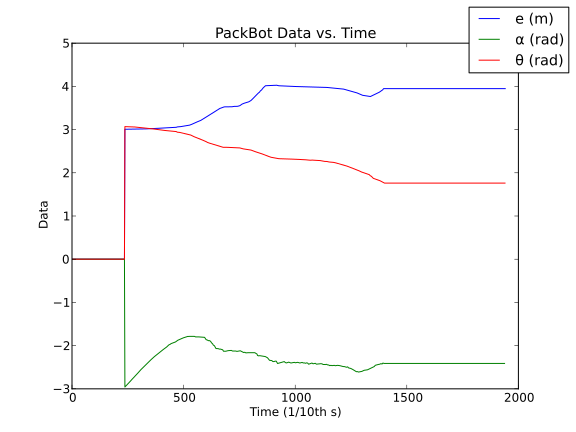
\includegraphics[width=.95\textwidth]{images/pbData}
	\caption{First attempt at running the PackBot using the Lyapunov controller.}
	\label{fig:lyapunovDataFirstAttempt}
\end{figure}
\chapter{Future Work}
*** Suggest avenues of study for future work. ***
\chapter{Conclusion}
*** Summarize the results here. ***
\appendices % Use \appendix for single, \appendices for multiple
\chapter{Source Code}
\label{ch:code}
*** Put source code here if applicable. Consider putting a list of Acronyms in an appendix. ***
\include{chapters/chAcronyms}

% Bibliography.
\bibliographystyle{these}
% \bibliographystyle{plain}
\bibliography{mybib}

\end{document}